\documentclass[12pt]{article}

\usepackage[hmargin=2.5cm, vmargin={3cm,3cm}, a4paper]{geometry} 
\usepackage{amsmath,amssymb,amsthm,mathrsfs}
\usepackage{epsfig,epsf,subfigure,graphicx,graphics}
\usepackage{float}
\usepackage{url,enumerate}
\usepackage{listings}
\usepackage{ragged2e}
\graphicspath{{fig/}}
\usepackage{fancyhdr}
\usepackage{hyperref}
\hypersetup{
    colorlinks=true,
    linkcolor=blue,
    filecolor=magenta,      
    urlcolor=cyan,
    pdfpagemode=FullScreen,
    }
\setlength{\headheight}{12pt}
\pagestyle{fancyplain}

\graphicspath{ {./images/} }%Path to the images
 
\rhead{}
\lhead{}
\chead{{\it Graph Signal Processing Course, ETSETB}}
\lfoot{}
\cfoot{\thepage}
\rfoot{}
\title{Practical session 2: Spectral Clustering}
\author{Gerard Castell and Victor Rubio}
\begin{document}
\maketitle

\thispagestyle{fancyplain}
\flushleft 


\Large
\hspace{10pt}
\small
\section{Link prediction: Lazega dataset}

%%Abstract Subsection
\subsection{Abstract}
\justifying
The link prediction problem aims at deciding whether there is an edge or not for the unobserved entries of the adjacency matrix $\mathbf{A}$. Existing link prediction models fall into two classes: unsupervised and supervised:
\begin{itemize}
    \item \textbf{Supervised methods} attempt to learn from a predetermined set, using the observed links as the training data.
    \item \textbf{Unsupervised models} compute scores for pairs of nodes based on topological properties of the graph. These models use predefined scores that are invariant to the specific structure of the input graph.
\end{itemize}
In this practice we want to try to use unsupervised methods observing the effect of different scores to the end result.

In order to compare the different scores used during the practice we will use the ROC measure; retaltionsip between Probability of Detection and the Probability of False Alarm.
%%First subsection
\subsection{Reading and cleaning up the data}
\justifying
After observing the information in the \href{https://www.stats.ox.ac.uk/~snijders/siena/Lazega_lawyers_data.htm}{dataset webpage} we can see that all files excep \textit{ELattr.dat} contain an adjacency matrix. The file \textit{ELattr.dat} contains attributes for each lawyer:
\smallskip
\begin{itemize}
    \item seniority
    \item status (1=partner; 2=associate)
    \item gender (1=man; 2=woman)
    \item office (1=Boston; 2=Hartford; 3=Providence)
    \item years with the firm
    \item age
    \item practice (1=litigation; 2=corporate)
    \item law school (1: harvard, yale; 2: ucon; 3: other)
\end{itemize}
\justifying
In order to collect the data we downloaded the files and wrote the following code:
\smallskip
\begin{lstlisting}[language=matlab]
%% Reading and cleaning up the data
    data = readtable('dataset/ELwork36.dat','ReadVariableNames',false);
    data_m=table2array(data);
    G=graph(data_m);

%Plot
    figure(1);
    plot(G)
    title('Original graph');
\end{lstlisting}
In the \href{fig:completeGraph}{figure bellow} we can observe the result of the execution of the previous code. 
\begin{figure}[H]
	\centering
	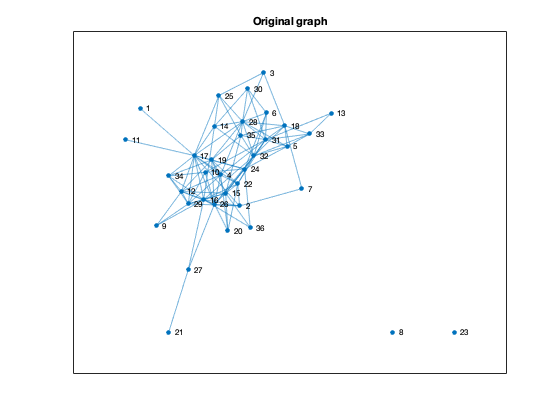
\includegraphics[width=13cm]{images/1.png}
	\caption{Plot of the graph built from the dataset \textit{ELwork36.dat.}}
	\label{fig:completeGraph}
\end{figure}

%Second subsection
\subsection{Common Neighbors}
\justifying
Once we have the original graph we want to remove some of the edges so we can start the procedure to predict the edges:
\smallskip
\begin{lstlisting}[language=matlab]
%% Common Neighbors
    X=ones(size(data_m,1));
    X=triu(X);
    X=X-diag(diag(X));
    [row, col] = find(X);
    rc=[row col]; %Row and col that are 1 (All possible edges in a graph)

    rnd_indexes = randperm(630, 630/5);
    rm = rc(rnd_indexes,:);%Random edges generated
    s_rm = rm(:,1);
    t_rm = rm(:,2);

    G_obs = rmedge(G,s_rm, t_rm);%Graph G removing the random edges

%Plot
    figure(2);
    plot(G_obs)
    title('Graph without 126 edges');
\end{lstlisting}
In the \href{fig:croppedGraph}{figure bellow} we can see the result of the execution of the previous code:
\begin{figure}[H]
	\centering
	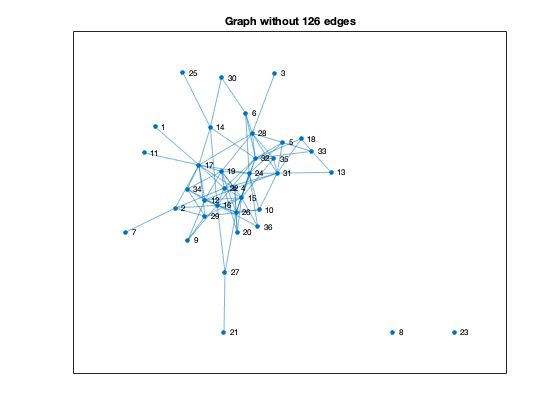
\includegraphics[width=13cm]{images/2.png}
	\caption{Plot of the graph removing $1/5$ of the edges.}
	\label{fig:croppedGraph}
\end{figure}

%Third subsection
\subsection{Score function}
\justifying
In order to determine what edges will be formed we define the matlab function $CNScoring(G, s, t)$:
\label{code:CNScoring}
\begin{lstlisting}
function score = CNScoring(G, s, t)
    %param s: is a scalar, source node
    %param t: is a scalar, target node
    %param G: is a graph
    s_neighbors = neighbors(G,s);
    t_neighbors = neighbors(G,t);
    CN = intersect(s_neighbors,t_neighbors);
    score=size(CN);
    score = score(1);
end
\end{lstlisting}
\justifying
This function will get a graph, a source node and a target node and find the number of non repeating neighbours that the two edges have in common. The function will return this value as the score.

Then we may introduce this function into our main code:

\begin{lstlisting}
th=5;
G_pred = G_obs;
predicted_true = [];

for i = 1:size(rm,1)%Changed rm for rc -> Score just for unknown edges
    disp(['Checking edge (', num2str(rm(i,1)), ',', num2str(rm(i,2)), ')']);
    score = CNScoring(G_obs, rm(i,1), rm(i,2));
    if score>=th
       disp(['Edge (', num2str(rm(i,1)), ',', num2str(rm(i,2)), ') is added...'])
       G_pred = addedge(G_pred, rm(i,1), rm(i,2), 1);
       predicted_true = [predicted_true; rm(i,:)];
    else
       G_pred = rmedge(G_pred, rm(i,1), rm(i,2));
    end    
end

%% Plot corrected
figure(3);
plot(G_pred)
title('Graph predicted');

\end{lstlisting}
\justifying
In the previous code we used the function \href{code:CNScoring}{CNScoring} to obtain the Common Neighbors index and if the scored value is over the defined threshold we will add that edge to the graph. Afterwards we plot the resulting graph to compare their shape.

The \href{fig:correctedGraph}{following figure} is the plot of the graph with the predicted missing edges: 
\begin{figure}[H]
    \centering
    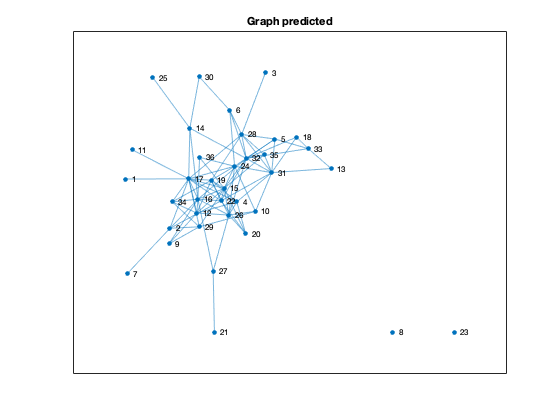
\includegraphics[width=13cm]{images/3.png}
    \caption{Graph with predicted edges}
    \label{fig:correctedGraph}
\end{figure}
%Fourth subsection
\subsection{Probability of detection and false alarm}
\justifying
After getting the new edges we want to find the probability of detection ($P_d$) and the probability of false alarm ($P_F$). 

\justifying
The $P_d$ is the probability that we correctly detect an existing edge from all of those edges that should exist.

\justifying
The $P_f$ is the probability of detecting an edge that should have weight 0 as an existing edge from all the edges that have weight 0. 

In order to calculate this probabilities we created the function \textit{CalcProbs}:

\begin{lstlisting}
function [PD,PF] = CalcProbs(th,G,rm, scoring)
    s_rm = rm(:,1);
    t_rm = rm(:,2);

    G_obs = rmedge(G,s_rm, t_rm);
    G_pred = G_obs;
    predicted_true = [];
    
    for i = 1:size(rm,1)
        score = scoring(G_obs, rm(i,1), rm(i,2));
        if score>=th
           G_pred = addedge(G_pred, rm(i,1), rm(i,2), 1);
           predicted_true = [predicted_true; rm(i,:)];
        else
           G_pred = rmedge(G_pred, rm(i,1), rm(i,2));
        end    
    end
    
    %% Probability of detection and false alarm
    [s_G, t_G] = findedge(G);
    [s_G_pred, t_G_pred] = findedge(G_pred);
    idx_G = [s_G, t_G];
    idx_G_pred = [s_G_pred, t_G_pred];
    
    predicted_true_1 = 0;
    for i = 1:size(predicted_true,1)
        for j = 1:size(idx_G,1)
            if all(predicted_true(i, :) == idx_G(j,:))
                predicted_true_1 = predicted_true_1 + 1;
            end
        end
    end
    
    to_be_true_1 = 0;
    for i = 1:size(rm,1)
        for j = 1:size(idx_G,1)
            if all(rm(i, :) == idx_G(j,:))
                to_be_true_1 = to_be_true_1 + 1;
            end
        end
    end
    
    predicted_false_1 = size(predicted_true, 1) - predicted_true_1;% All predicted as 1 minus the real predicted as 1;
    to_be_false_0 = size(rm,1) - to_be_true_1;
    PD = predicted_true_1/to_be_true_1;
    PF = predicted_false_1/to_be_false_0;

end
\end{lstlisting}

%Fifth subsection
\subsection{Receiving Operating Characteristic (ROC) curve}
\justifying
In order to calculate the ROC we will define a range of thersholds, from 1 to 8 and check the relationship between the $P_d$ and $P_f$ values.

We used the follwoing code to plot the ROC:
\begin{lstlisting}
th_table = [];
for i=0:0.05:10 
    [PD, PF] = CalcProbs(i,G,rm, @CNScoring);
    th_table = [th_table; PD PF];
end
figure(4);
plot(th_table(:,2), th_table(:,1));
title('ROC with Common Neighbors index')
\end{lstlisting}

%Sixth subsection
\subsection{Other link prediction methods}
Finally we want t test different scorings in the edge selection part of the practice. Following the slides from the coure we selected the Jaccard and the Adamic-Adar indexes. 
\subsubsection{Jaccard index}
\justifying
The Jacard index is based on the relationship between the intersection of the common nodes between source and target nodes and the union of said nodes. In order to use this index as our scoring we created the function $JScoring(G,s,t)$.
\begin{lstlisting}
function score_J = JScoring(G,s,t)
%param s: is a scalar, source node
%param t: is a scalar, target node
%param G: is a graph
    score_CN = CNScoring(G,s,t);
    s_neighbors = neighbors(G,s);
    t_neighbors = neighbors(G,t);
    U=union(s_neighbors,t_neighbors);
    size_U = size(U,1);
    score_J = score_CN/size_U;
end
\end{lstlisting}

\subsubsection{Adamic–Adar index}
\justifying
The Adamic-Adar index calculates the logarithm of the degree of the nodes that are an intersection between source and target nodes. After that we will create a sum of the inverse of those logarithms. IN order to calculate this index we created the function $AAScoring(G,s,t)$
\begin{lstlisting}
function score_AA = AAScoring(G,s,t)
%param s: Source node
%param t: Target node
%param G: Graph
    s_neighbors = neighbors(G,s);
    t_neighbors = neighbors(G,t);
    isec = intersect(s_neighbors,t_neighbors);
    score_AA = 0;
    for i = 1:size(isec,1)
        d = degree(G, isec);
        score_AA = score_AA + 1./log(d);
    end
end
\end{lstlisting}

\subsection{Results and comparisons}
Finally, we have plot the 3 indexes that we have developed in the same graph, as you can see below. As we know, in a ROC space a Perfect classifier would be and the top-left corner, whilst the worst would be at the bottom-right. The diagonal function represents a random classifier, with a 50\% of probability to classify true or false.\\

The Area Under the Curve, well-known as AUC, is crucial to evaluate the performance of a classifier. The higher the AUC is the better the classifier performs. That said, the we may observe that our three predictors have better performance than a random classifier, since the are they take is bigger, so the predictor that we have developed in this practice works good.

\begin{figure}[H]
    \centering
    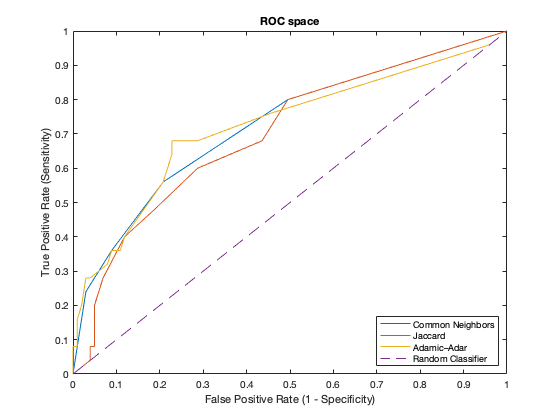
\includegraphics[width=13cm]{images/4.png}
    \caption{Comparison between the ROCs calculated during the practice}
    \label{fig:ROCComparison}
\end{figure}

When we want to focus on which index works better for our task, we should calculate their AUC and take the biggest one, but at first glance we can think that the Adamic-Adar index works slightly accurate. Even though, we have calculated the AUC for each curve and the result is the following table:\\

\begin{center}
\begin{tabular}{ | c | c | }
\hline
  Index & AUC \\ 
\hline
\hline
 Common Neighbors & 0.7257 \\  
 \hline
 Jaccard & 0.7006 \\  
 \hline
 Adamic-Adar & 0.6844  \\
\hline
\end{tabular}
\end{center}

The areas calculated with Matlab reveal that the better classifier is the Common Neighbors in our case. However, this is not supposed to be a generic solution since it strongly depends on the data for each problem and in our practice also depends on the random edges removed from the initial Graph, which also can affect to the final results.

In conclusion, the three link predictors have shown a good performance and quite similar between them so the practice has been carried out successfully.

\end{document}